% HCI - Assignement III
% Karthikeya Udupa K M (1393456)
\documentclass[10pt,a4paper]{article} 
\usepackage[scale=0.8]{geometry} % adjust the page margins
% The document preamble 
%\usepackage{times} 
\usepackage[utf8]{inputenc} 
\usepackage{graphicx}
%\usepackage{chicago}

% Details of the titlepage 
\title{Physicality (Assignment 3) } 
\author{Karthikeya Udupa K M, Oliver Smithson, Yegana Abdullayeva} 
\date{\today}

\begin{document} 

\maketitle
\noindent


\section{Device}
The device is a compact and portable speaker with a 40mm driver creating the audio output. It is capable of receiving input in the form of electric signal from the 3.5mm audio connector. The device has a rechargeable battery which can be charged through the mini-usb port available on the device. The power supply to the device can be controlled by the ON/OFF switch, toggling of which also controls the LED which indicates the present state of the device. The device also consists of a manually expandable vacuum that allows the volume and the bass of the audio output to be increased. The device also has a 3.5mm audio connector which allows to connect many of these devices in parallel.

The functioning of the device is similar to any speaker device, which is a electroacoustic transducer, which when provided electrical audio signal input through the input mode (3.5mm slot) create a magnetic field in the coil and making it move, which in turn creates the sound. The internal state of the device is essentially altered based on the electrical signal being supplied through the input. 

\section{Controls}
\begin{figure}[hbpt]
\centerline{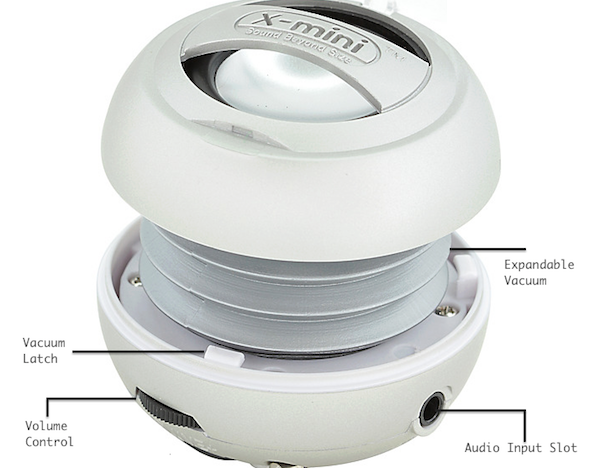
\includegraphics[width=15cm,height=10cm,keepaspectratio]{DW1}}
\caption {The portable speaker with the various components marked.}
\label{physical_state_power_switch}
\end{figure}
%-- -- -- -- -- -- -- -- -- -- -- --%
\subsection{Power Switch}
It is a toggle switch controlling the power supply to the device from the internal battery. There is a LED which indicates the current state of the device by providing a visual feedback when the switch is toggled.

\begin{figure}[hbpt]
\centerline{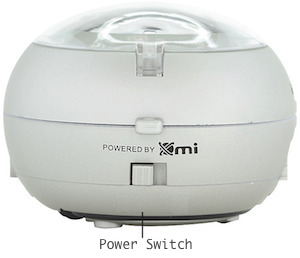
\includegraphics[width=200px,height=158px,keepaspectratio]{DW2}}
\caption{The power switch of the device.}
\label{physical_state_power_switch}
\end{figure}

\subsection{Physical Interaction in `Unplugged State'}

The power switch is a manual control which can be toggled by moving it either left or right to alter its state. The physical movement of the switch provides a direct feedback to the user, letting him know that the state has changed. This is also indicated by the switch's inability to move forward in the particular direction any further once the state has been changed. The notation above the switch indicates the present state of the switch more evidently to the user. 

\begin{description}

\item [Physical Manipulation] is done by asserting pressure on the switch towards the proper direction (one with space available ahead of the switch for movement). There is a certain amount of pressure that has to be exerted before the state of the switch changes.

\item [Possible Physical States] for the control are LEFT and RIGHT.

\item [Direct Physical Feedback] is provided by the feeling of movement of the switch which the user feels when he changes the state and also the inability to move the switch any further once the state has been changed.
\end{description}


\begin{figure}[hbpt]
\centerline{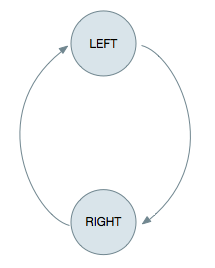
\includegraphics[width=5cm,height=7cm,keepaspectratio]{PW1}}
\caption{Physical state representation for a Power Switch}
\label{physical_state_power_switch}
\end{figure}


\subsection{Effects on Internal States in `Plugged State'}


The switch controls the flow of electricity to the electronic components in the device. The device has an internal battery which is rechargeable through the mini-usb slot, when its charged and the switch is turned on, the power is provided to the coils, which creates the magnetic field hat is required to create the audio output when provided with the input signal. To indicate the state an additional LED is provided which is turned on when the switch is in the ON state.

\begin{description}

\item [Secondary Feedback] is provided by the LED light, which is turned on (Physical feedback) and the audio is generated by the speakers (virtual feedback) if the input signal is provided.
\item [Logical State] that would correspond to the control's state is ON and OFF.

\end{description}

\subsection{Formal Representation}

\begin{figure}[hbpt]
\centerline{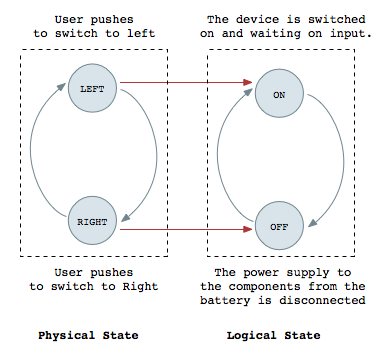
\includegraphics[width=381px,height=300px,keepaspectratio]{PW2}}
\caption {The mapping of the physical and internal states.}
\label{physical_state_power_switch}
\end{figure}

\noindent
As we can see the switch controls the working state of the device directly, this relation can be represented as the below mentioned pseudo code.
\begin{center}
\begin{verbatim} 

IF SWITCH_STATE == LEFT
     DEVICE_STATE == ON
ELSIF SWITCH_STATE == RIGHT
     DEVICE_STATE == OFF
ENDIF

\end{verbatim} 
\end{center}
%-- -- -- -- -- -- -- -- -- -- -- --%
\section{Volume Control}
A semi-circular dial which allows to control the level of the volume output generated by the device using a resistive circuit to control the flow of current. The dial does not have any marking to indicate the current level of volume but on movement from left to right increases the volume output. The dial is created with minute groves to provide easier control/grip while rotating.


\subsection{Physical Interaction in `Unplugged State'}

As mentioned above the dial can be rotated in either direction. The movement can only be done to a certain extent after which the dial can be moved no further in that particular direction.

\begin{figure}[hbpt]
\centerline{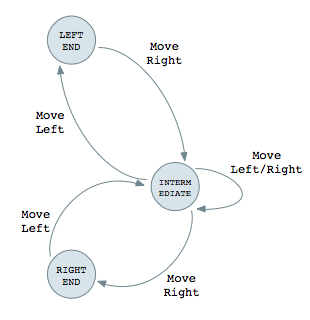
\includegraphics[width=280px,height=300px,keepaspectratio]{VC1}}
\caption {Volume Control: The physical states and transition between then.}
\label{physical_state_power_switch}
\end{figure}

\begin{description}
\item [Physical manipulation] is done by rotating the dial through assertion of force in a certain direction. The rotation can be either towards left or right.
\item [Physical state] is changes on rotation of the dial, the states can be classified as follows:
\begin{itemize}
\item Left End State (Cannot move to left any further.)
\item Right End State (Cannot move to right any further.)
\item Intermediate Rotatory State (Can move either left or right. The control remains in this state until either moving left or right has taken it to a state where it cannot move any further in which case the state of the device would change to Left or Right End state.)
\end{itemize}
\item [Direct physical feedback] is provided through the feeling of movement of the wheel which is felt by the user. The groves in the dial gives additional feedback to control the dial more effectively.
\end{description}

\subsection{Effects on Internal States in `Plugged State'}
Movement of the dial towards the right increases the volume to the device (reducing the resistance in the flow of current to the components). The left most state of the dial indicates maximum resistance hence the least amount of sound is produced whereas the rightmost state indicates minimum resistance so maximum volume is produced. Intermediate state where the dial can be rotated either way produces sound based on its position.

\begin{description}

\item [Secondary Feedback] is provided by change in the auditory response provided by the device almost instantaneously when the dial is rotated.
\item [Logical State] that would correspond to the control's internal state is the minimum or maximum volume output (digitally achievable) of the device along with an intermediate state which would be a combined representation of all the other levels of volume which are nor minimum or maximum and the volume can either be increased or decreased from that level.

\end{description}

\subsection{Formal Representation}

\begin{figure}[hbpt]
\centerline{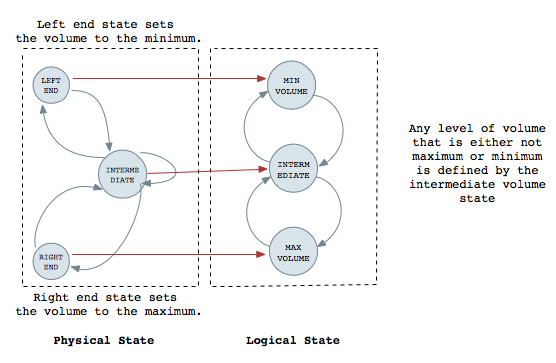
\includegraphics[width=556px,height=300px,keepaspectratio]{VC2}}
\caption {The mapping of the physical and internal states.}
\label{physical_state_power_switch}
\end{figure}

\noindent
The volume control alters the volume based on the direction of rotation to an extend that the volume can be changed no further. The pseudo code below demonstrates the same.
\begin{center}
\begin{verbatim} 

IF ROTATE_DIRECTION == LEFT
   IF VOLUME_LEVEL <> MINIMUM_VOLUME
      VOLUME_LEVEL = VOLUME_LEVEL - 1
   ENDIF
ELSIF IF ROTATE_DIRECTION == RIGHT
   IF VOLUME_LEVEL <> MAXIMUM_VOLUME
      VOLUME_LEVEL = VOLUME_LEVEL + 1
   ENDIF
ENDIF

\end{verbatim} 
\end{center}

%-- -- -- -- -- -- -- -- -- -- -- --%
\section{Expandable Vacuum}
The device has an expandable section that allows it to boost the volume and the bass output of the device. The control consists of two components, the first component is a latch which holds the expandable section in place when closed. The second component is the expandable section which links the two halves of the device, when expanded a vacuum is formed between both the halves inside the expanded area. 


\subsection{Physical Interaction in `Unplugged State'}

The expansion is controlled by a latch that can be opened by twisting the two haves of the device. on twisting the top half anti-clockwise, the latch is unlocked and the section that links the two part which is vacuum expands hence increasing the size of the device and creating a vacuum tube between the two halves. The device can be restored to the original state by exerting the pressure from the top to compress the expandable section in between and then twisting the top clockwise to close the latch. If the section is left in an intermediate state without locking, it expands and restores to the previous state.


\begin{figure}[hbpt]
\centerline{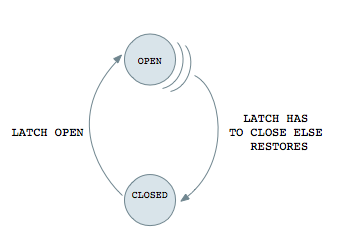
\includegraphics[width=280px,height=300px,keepaspectratio]{EV1}}
\caption {Expandable Vacuum: Physical states.}
\label{physical_state_power_switch}
\end{figure}

\begin{description}

\item [Physical manipulation] is done by rotating the two halves and to lock and unlock the latch. To change the state, pressure would be required to be exerted from the top to close the expanded section and then rotated clockwise to complete the state transition.
\item [Physical state] of the device would be Open and Closed state.
\item [Direct physical feedback] is provided through the feeling of movement of the latch and the visual change in the device's state by the expansion of the vacuum section.
\end{description}

 
\subsection{Effects on Internal States in `Plugged State'}
The device's internal state is not digitally modified by the control however the control has an effect on the internal state and the output of the device when it is ON. The purpose of the control is to open the expandable section which allows the audio output of the device to have more vacuum space below the diaphragm and coil to produce increased amount of bass and volume output.

\begin{description}
\item [Secondary Feedback] is provided by change in the auditory response, both as volume and bass, provided by the device when the section is expanded.
\item [Logical State] that would correspond to the control's internal state is the maximum or minimum volume and bass for a provided digitally preset value of volume (through the dial).
\end{description}

\subsection{Formal Representation}

\begin{figure}[hbpt]
\centerline{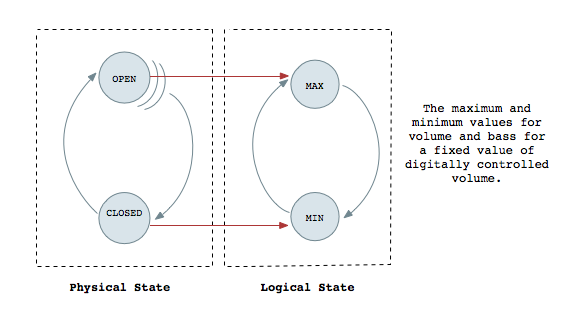
\includegraphics[width=556px,height=300px,keepaspectratio]{EV2}}
\caption {The mapping of the physical and internal states.}
\label{physical_state_power_switch}
\end{figure}

\noindent
The expandable vacuum control alters the volume and bass based on the state of the control, this expansion alters the volume and bass by a certain amount when at a certain digital volume level. 
%-- -- -- -- -- -- -- -- -- -- -- --%
\end{document} 

